% Copyright 2024- Jay Jay Billings. Some rights reserved.
\documentclass{article}
\usepackage{graphicx} % Required for inserting images
\usepackage{hyperref}
\usepackage{tabularx}

\title{Learning to weld}
\author{Jay Jay Billings, Ph.D.}
\date{\today}

\begin{document}

\maketitle

I recently joined \href{https://makersmiths.org/}{Makersmiths}, a community forge and makerspace. I heard about Makersmiths in passing before moving to northern Virginia, and I was as happy as a school kid when I found that their Purcellville space was close to my house. My wife and I put it on our list to join, and recently, she urged me to sign up when I started talking about building a bridge to cross our creek. I'll cover the bridge in a later blog, but basically, I need to build a bridge big enough to support my tractor across a 17-32ft span, depending on where I build the bridge. This will require some very heavy steel, fin plates, huge bolts, and a lot of welding.

I won't cover Makersmiths in detail here, mostly because it is thoroughly discussed on our excellent website and \href{https://makersmiths.org/Blog}{blog}. But I really want to share what I learned in an excellent three-hour welding class on metal-inert gas welding that I finished last night! 

My first experience with welding was using a ``stick'' welder in my Dad's junkyard as a kid. It was rare that we used a welder because we were mostly cutting things to length for the smelter. Cutting was straightforward - and really fun! - using a reciprocating saw, a chop saw, or an oxyacetylene torch. Dad was masterful with the torch and was allegedly a superb welder, according to everyone in the yard. One fine day, he proved it and then gave us boys a quick lesson. Fast forward... a rather long time... and all I've done with welding since is simulate melt pools for work (arguably quite cool). I have soldered quite a bit, but any comparison between the physics of those two processes is outweighed by the difference in scale, in my opinion. So, when the metal inert gas welding course came up so soon after we joined, it looked like a great opportunity to get a jump start on building the skills I'll need to build the bridge.

\section*{Metal Inert Gas Welding}

Metal In

\section*{The Equipment}

\subsection*{Plasma Cutter}

\subsection*{MIG Welder}

Fire brick

\subsection*{Clothes}

\section*{Welds}

I did a test weld.

\subsection*{Butt Weld}

\begin{figure}[h]
\caption{Front side of my butt weld. The weld path goes from left to right.}
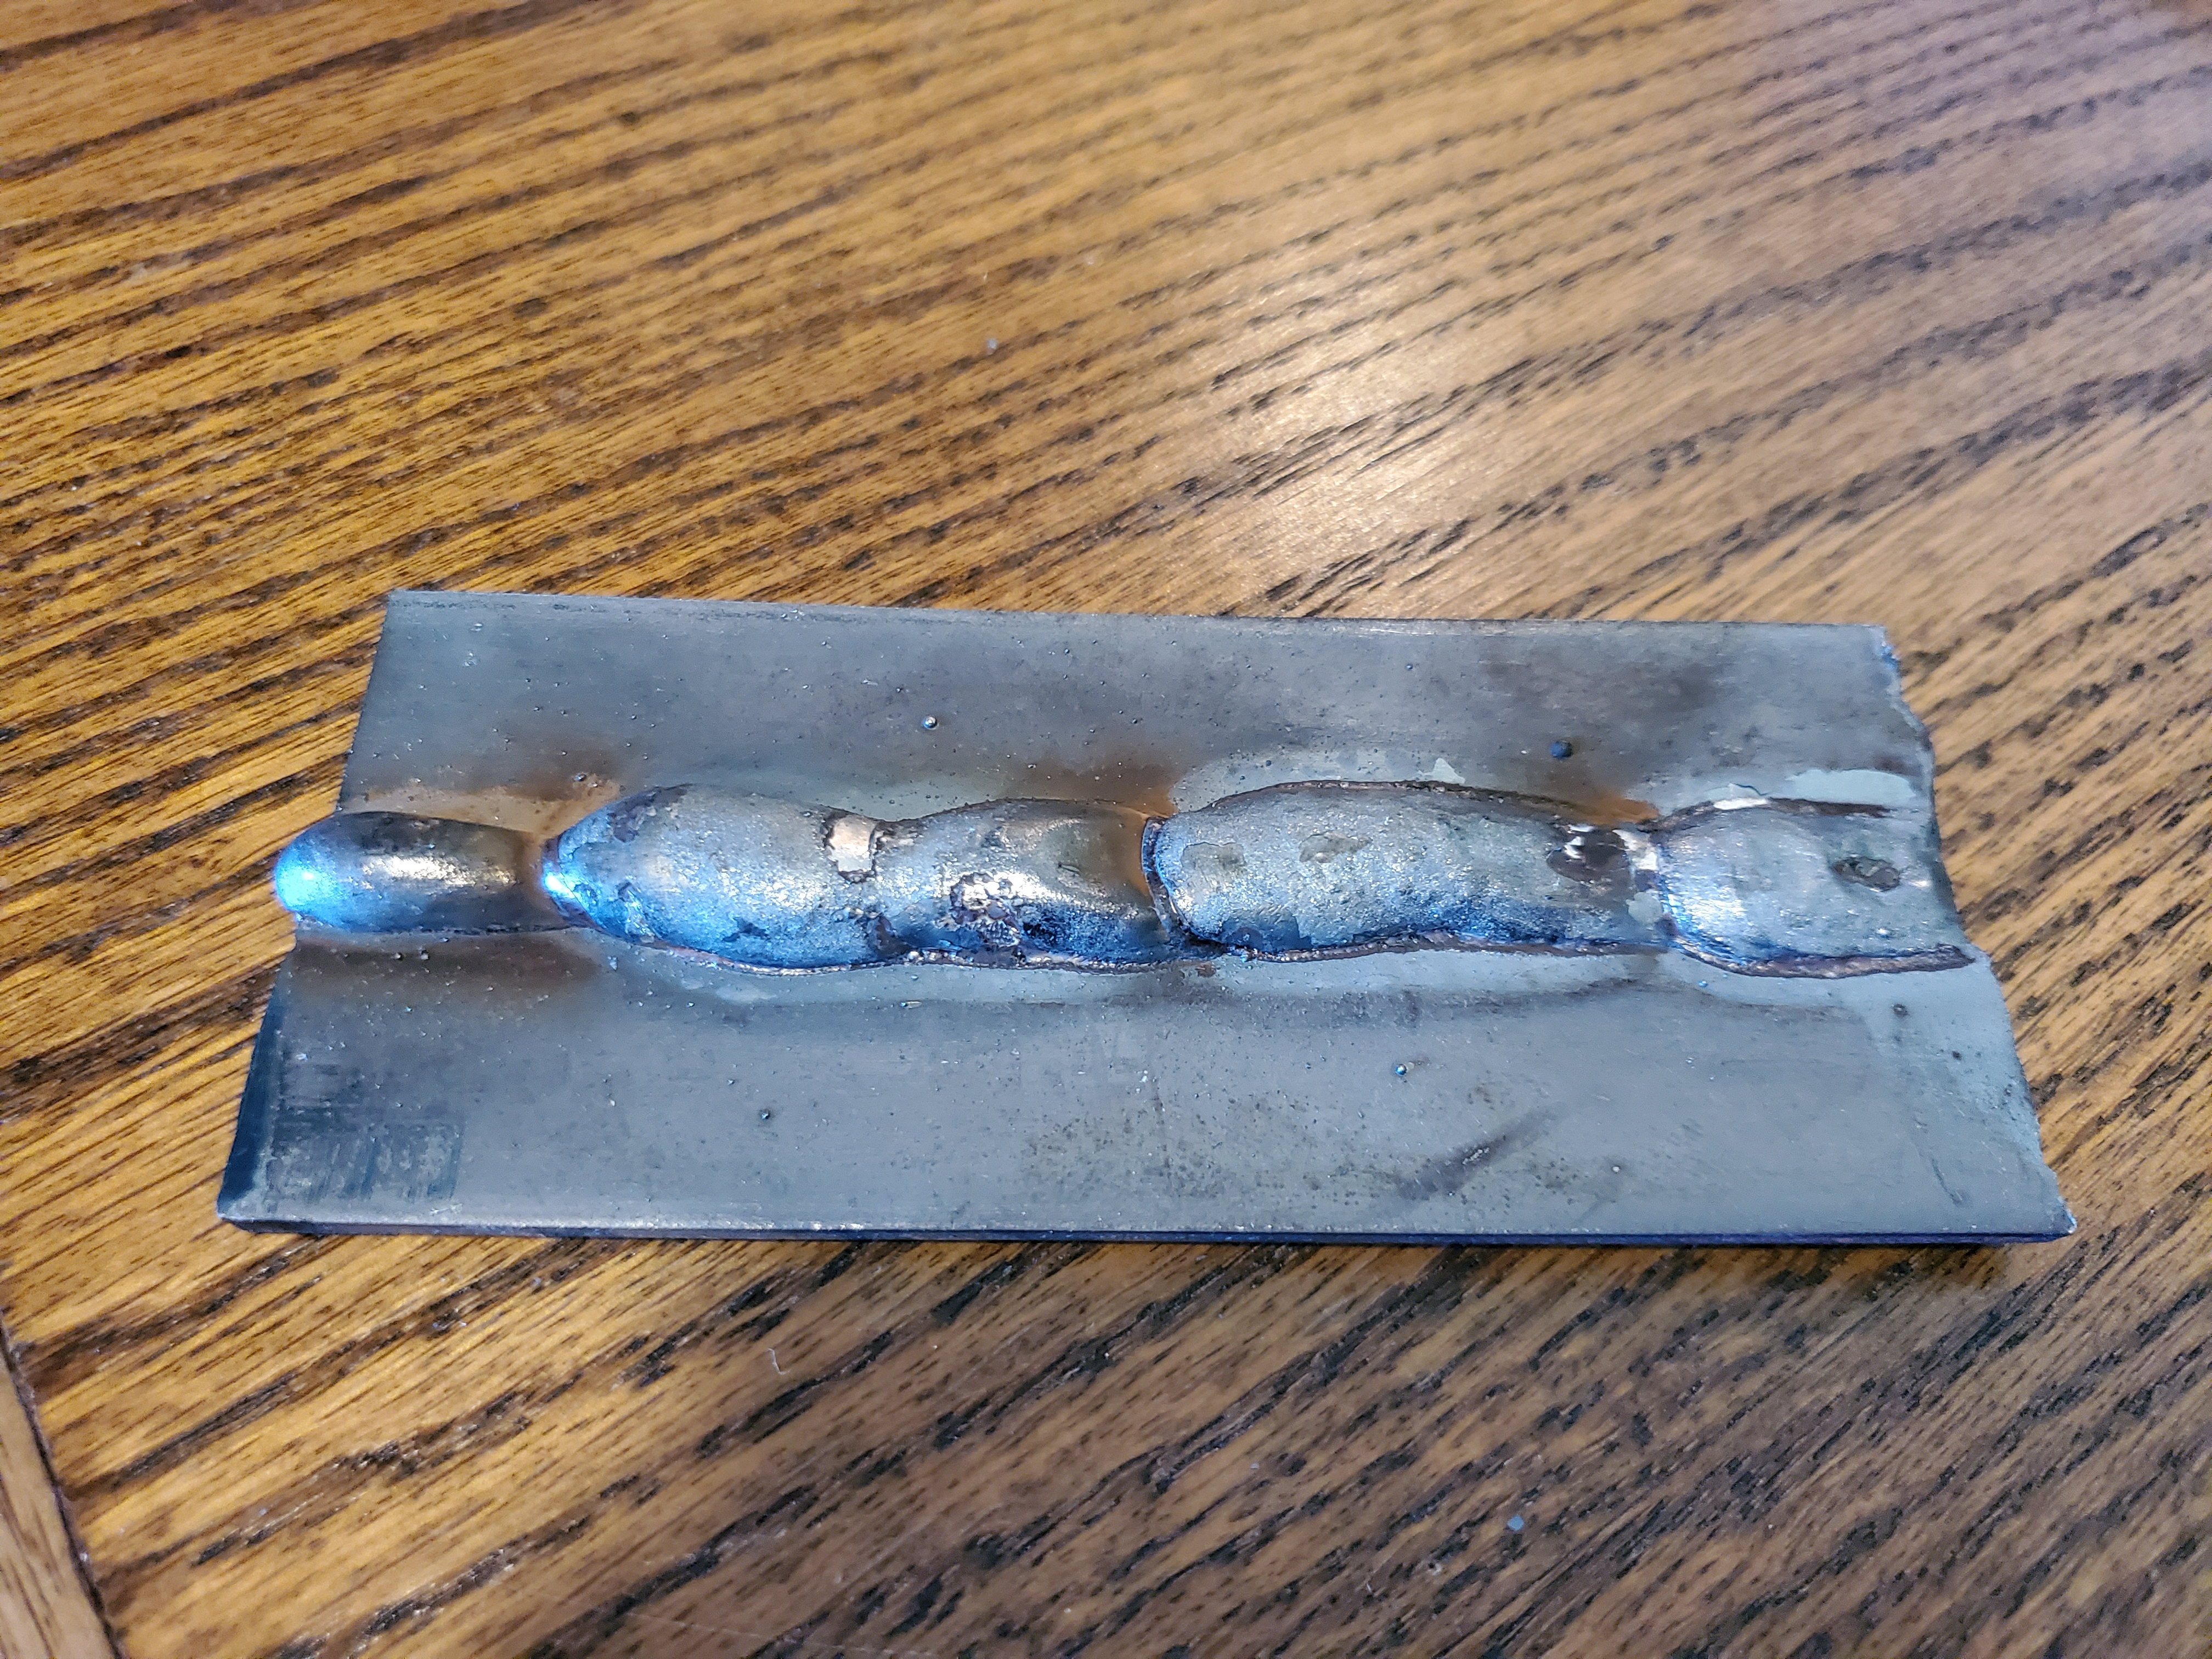
\includegraphics[width=\textwidth]{assets/buttWeldFront_20240229.jpg}
\end{figure}

\begin{figure}[h]
\caption{Back side of my butt weld with the weld path going from left to right.}
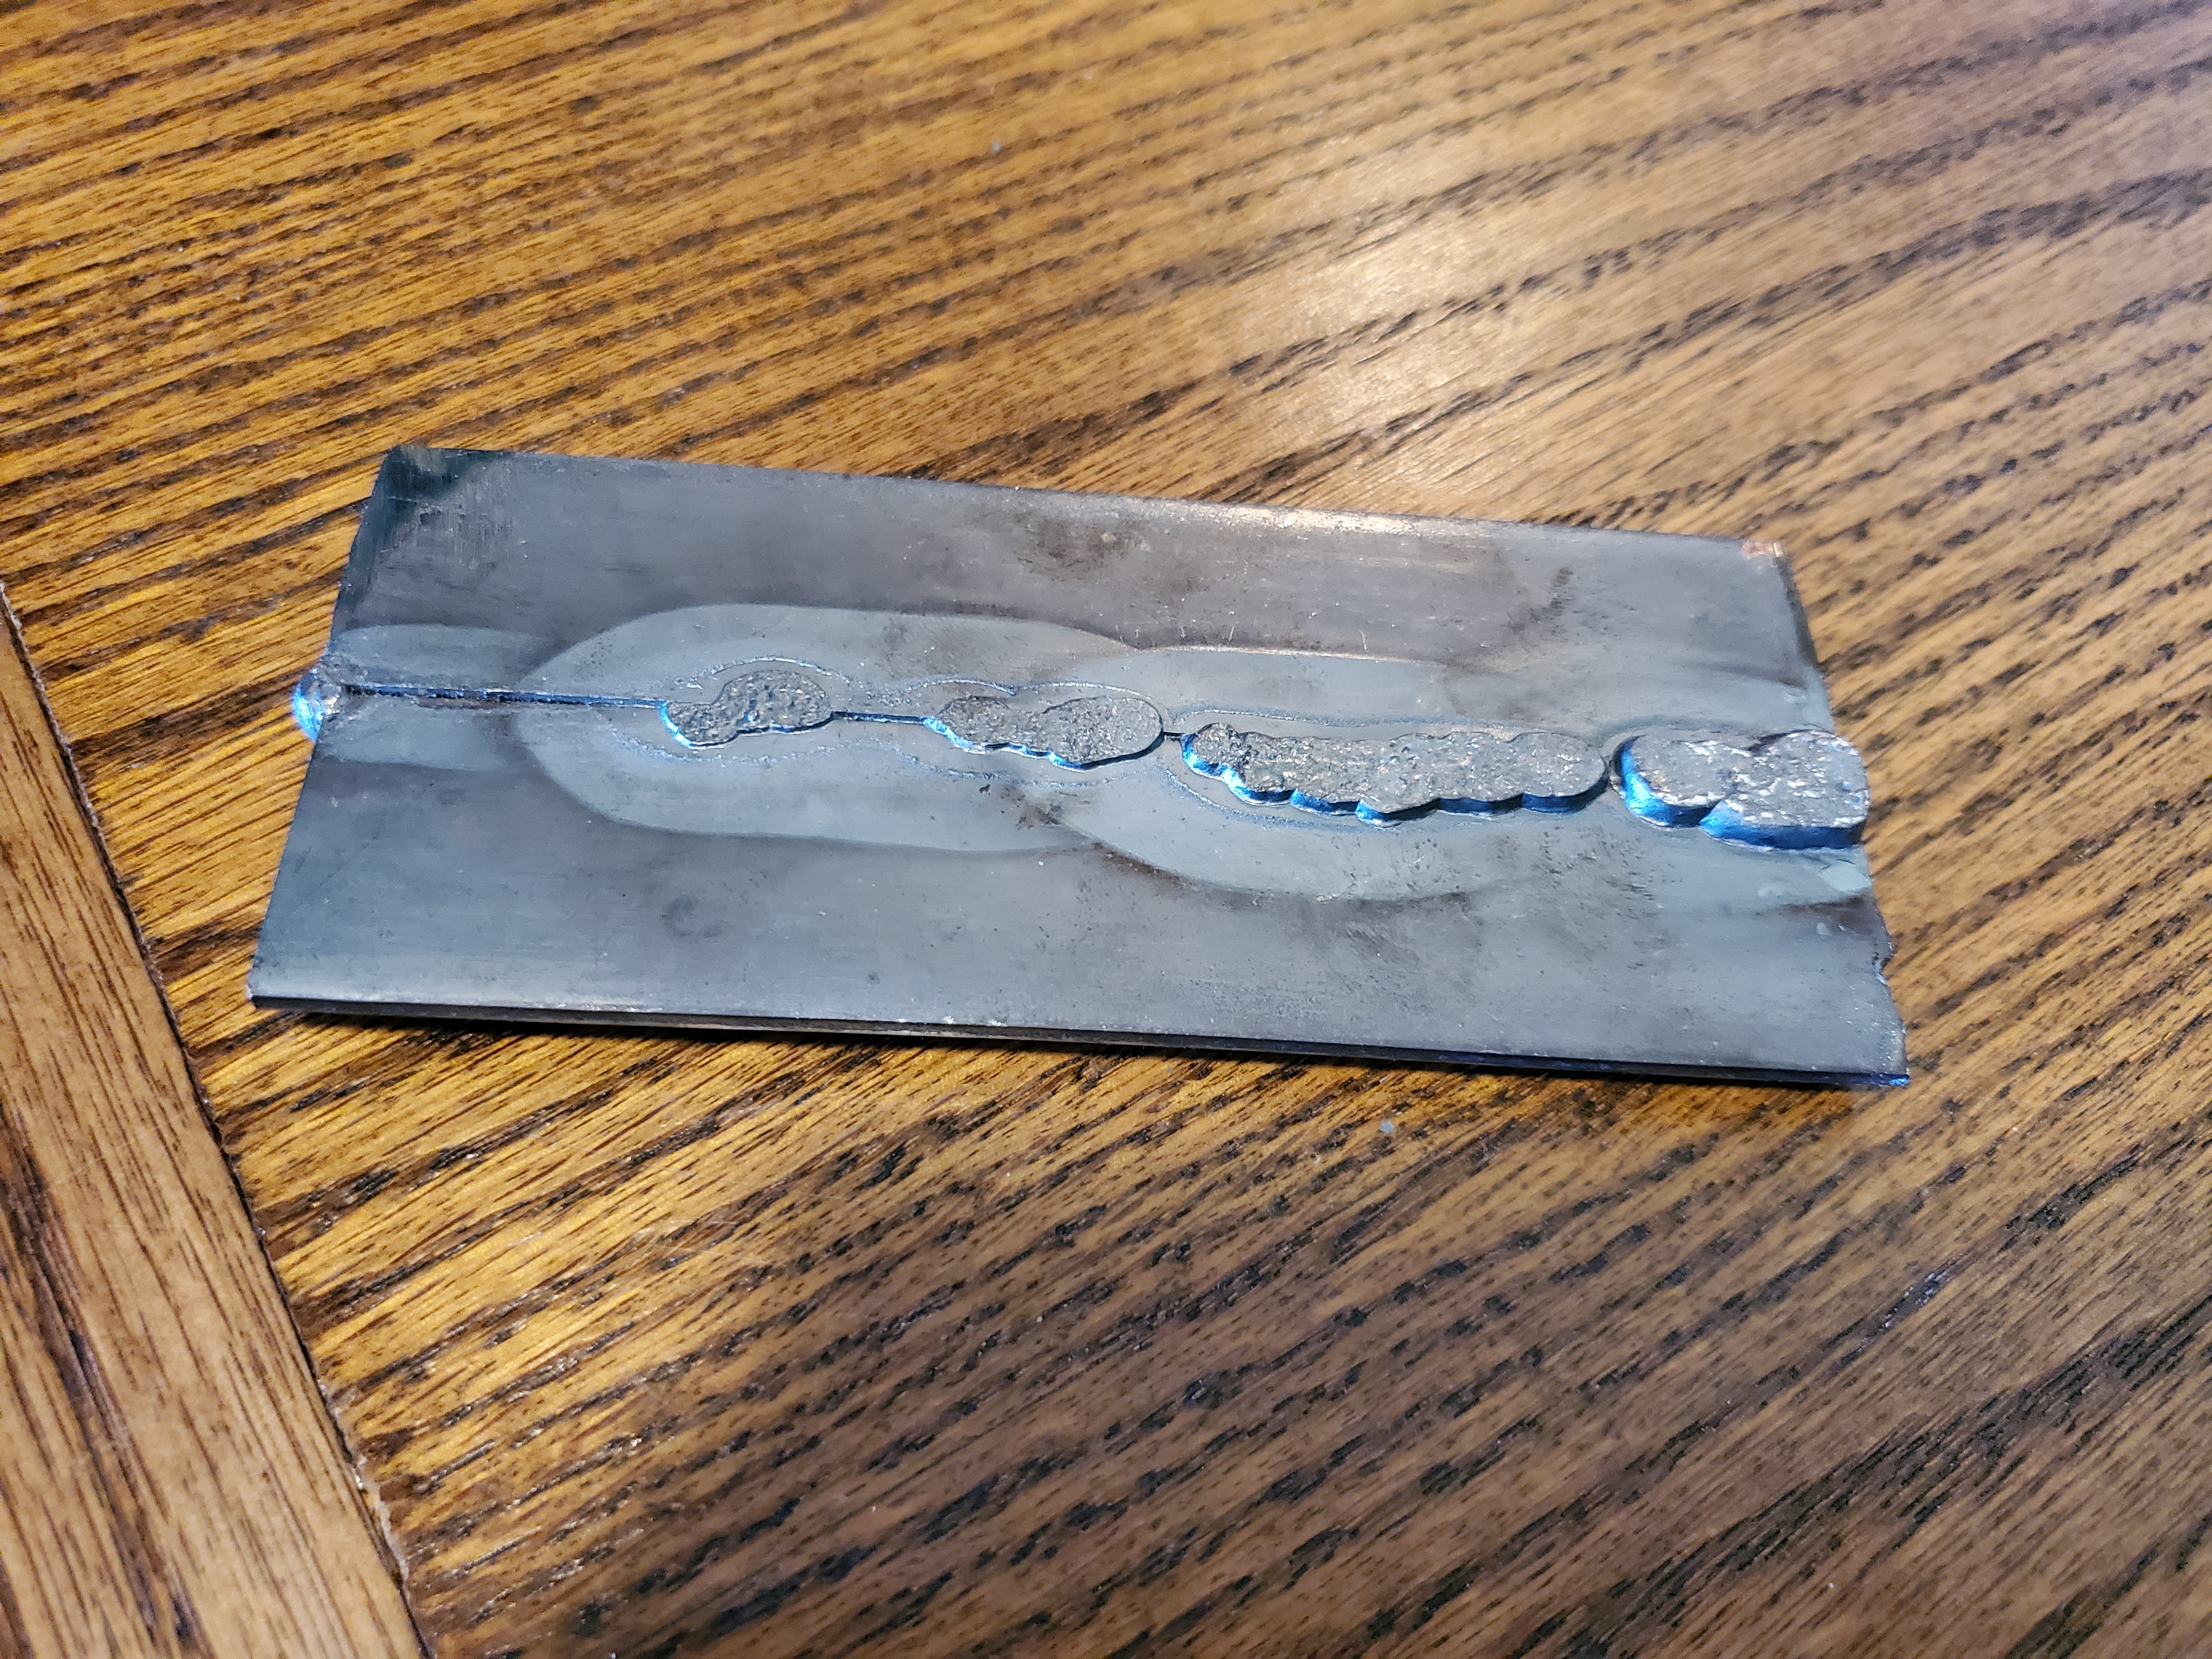
\includegraphics[width=\textwidth]{assets/buttWeldBack_20240229.jpg}
\end{figure}

\subsection*{Corner Weld}

\begin{figure}[h]
\caption{The front/inside of my corner weld showing a blown out corner (see next picture), two tacks, and a weld path from left to right.}
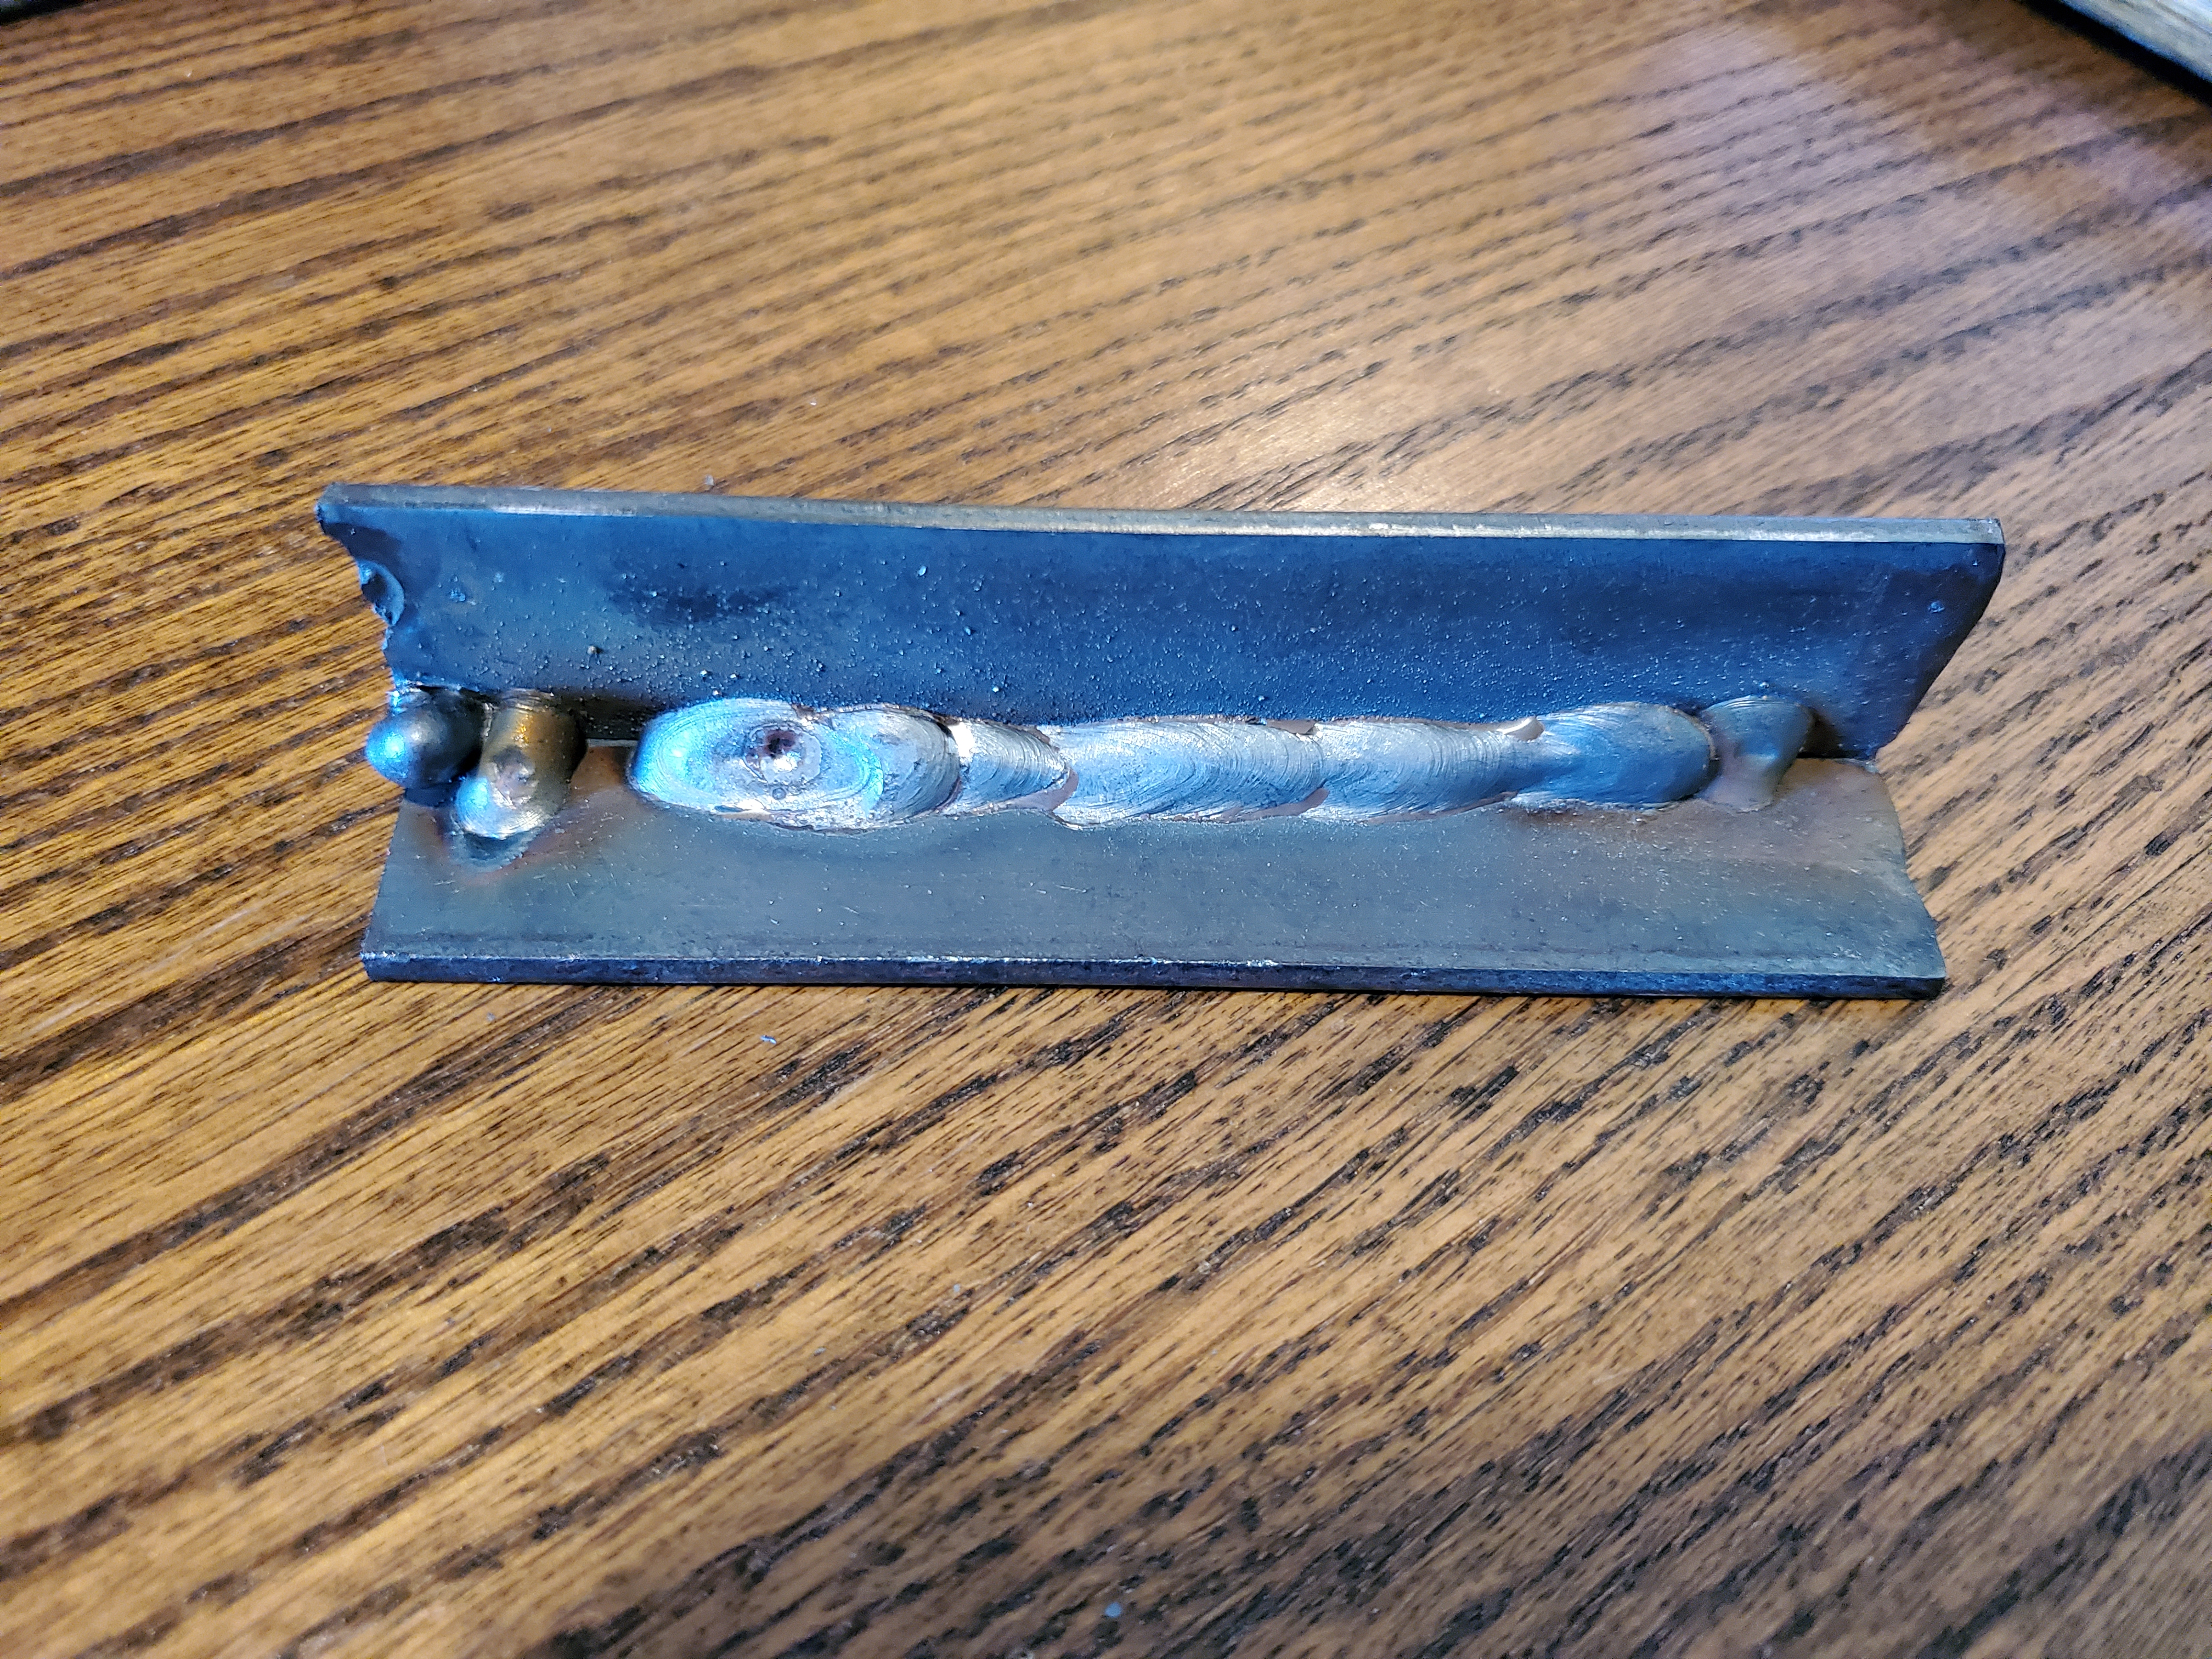
\includegraphics[width=\textwidth]{assets/cornerWeldFront_20240229.jpg}
\end{figure}

\begin{figure}[h]
\caption{The outside of the corner weld with the weld path going from left to right. The blown-out corner is visible on the left, and the weld gets smaller and smoother to the right as we decrease the feed rate and voltage.}
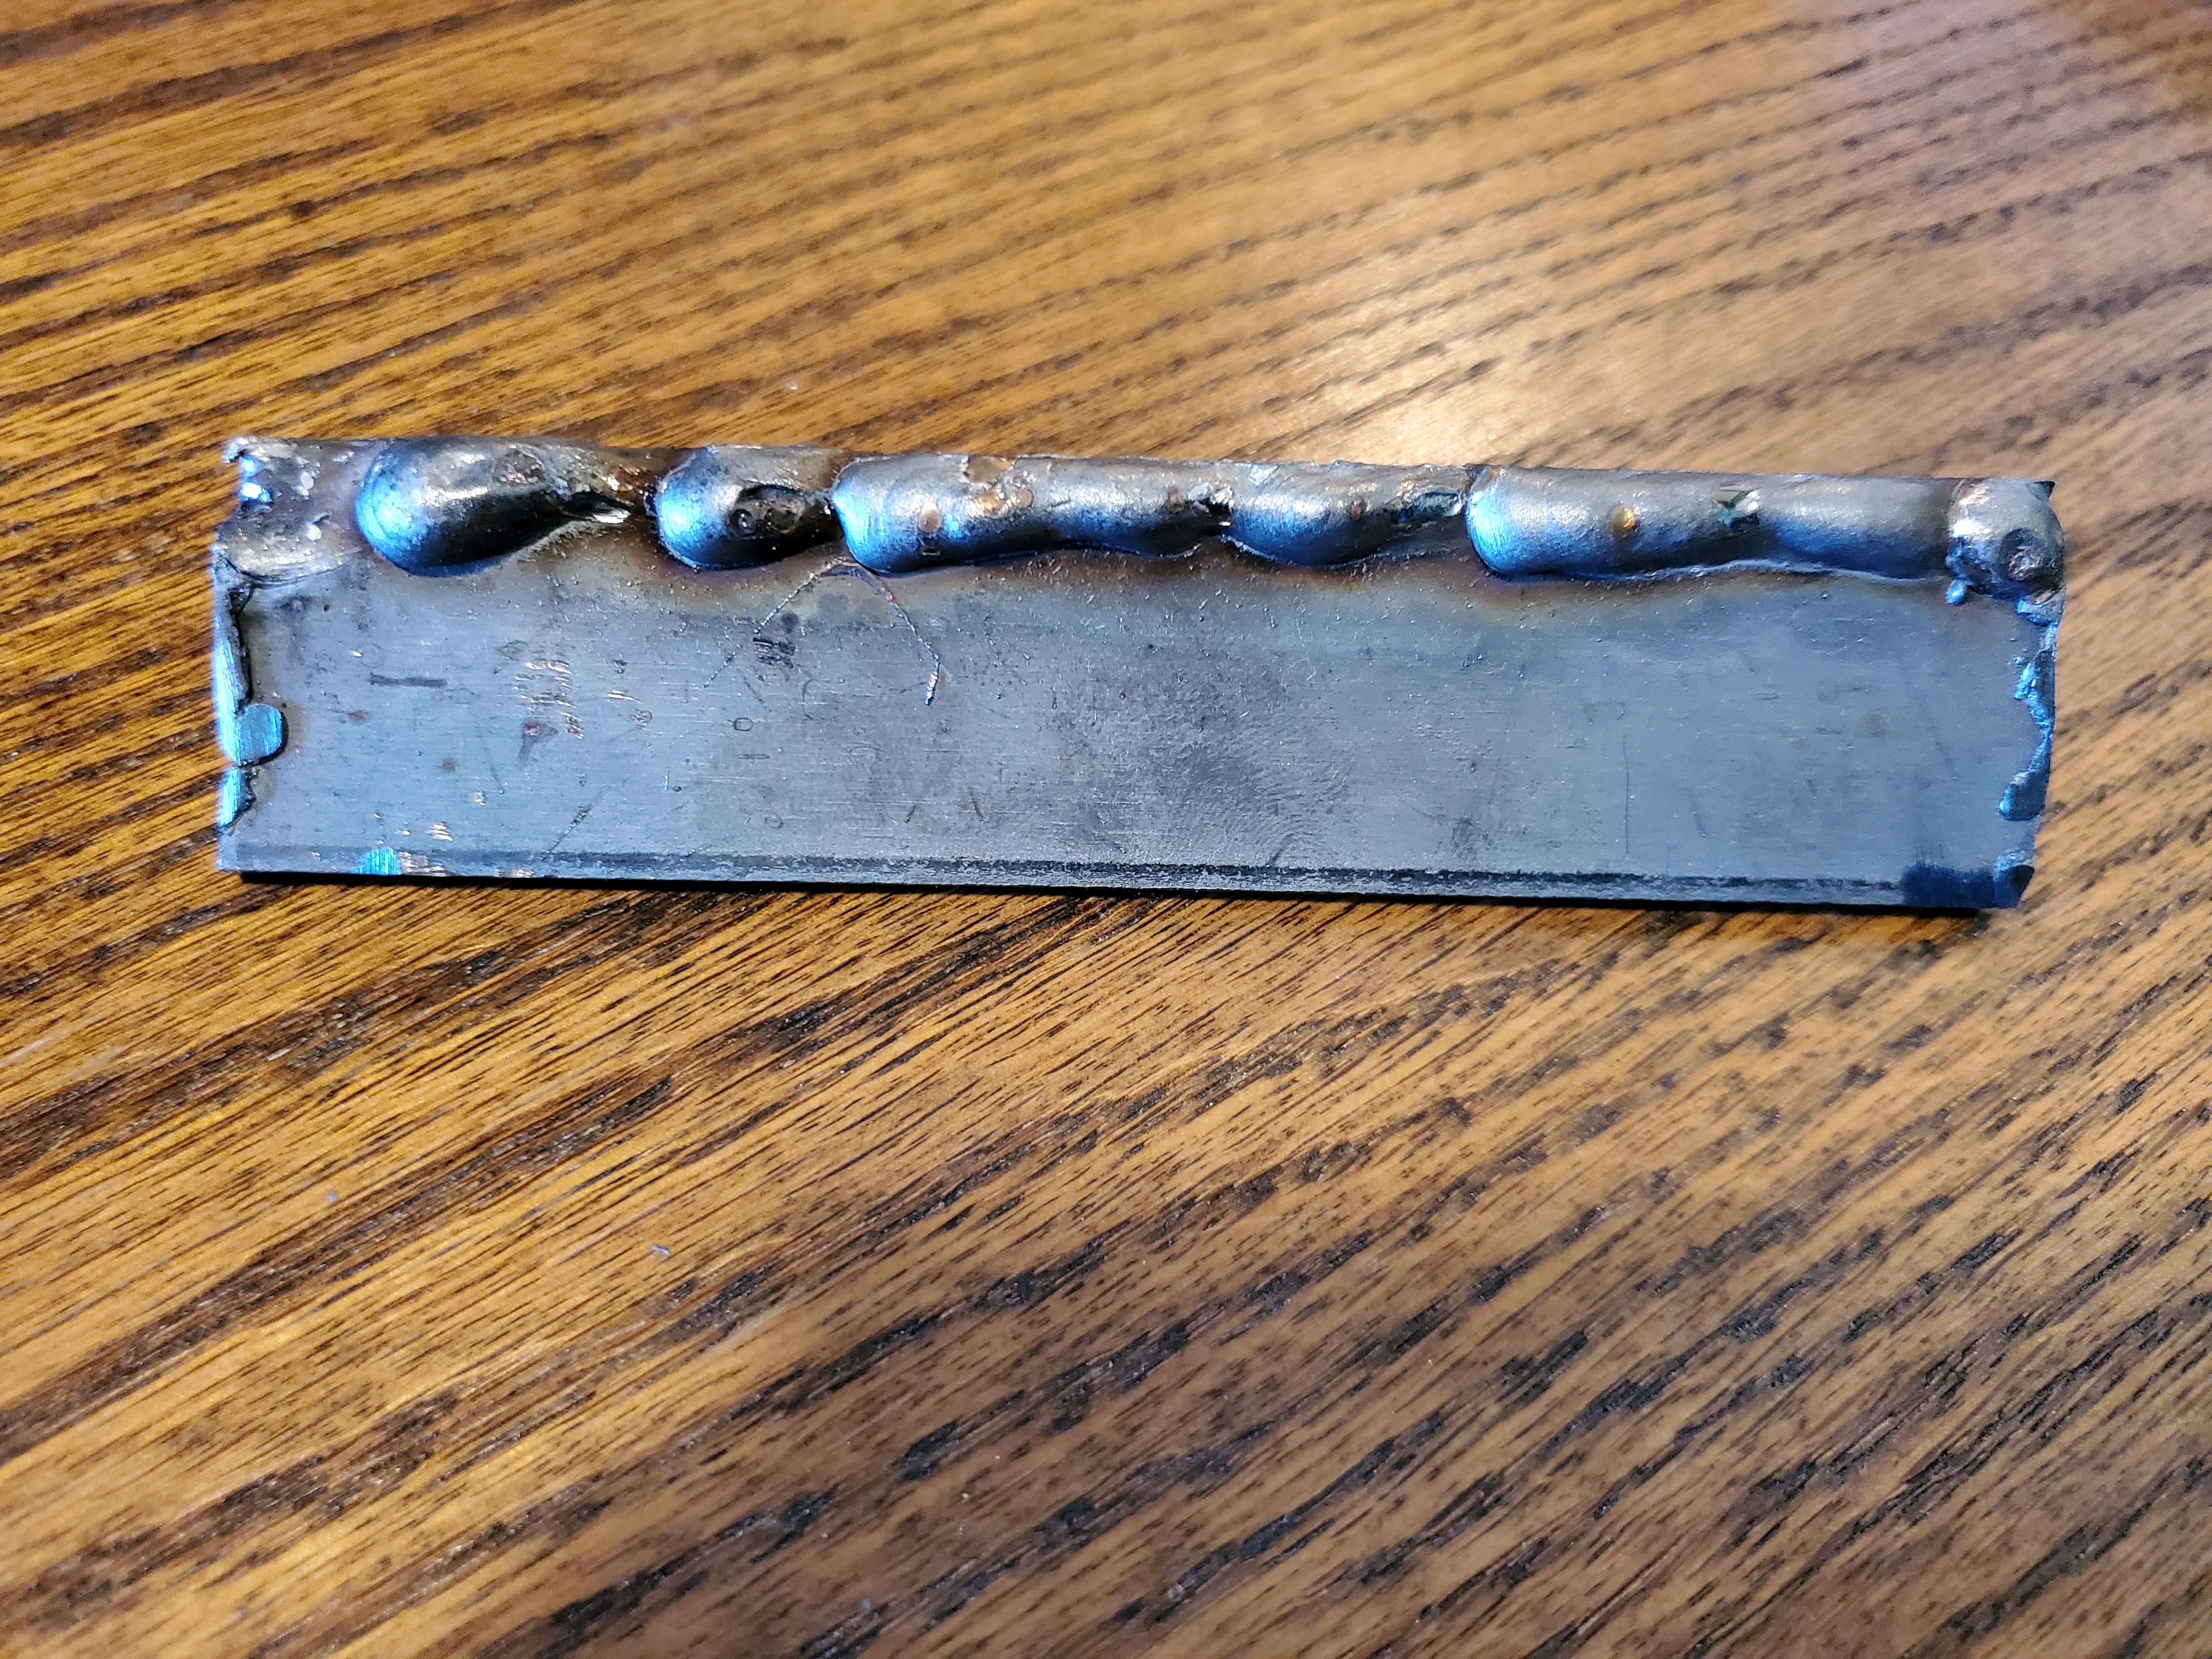
\includegraphics[width=\textwidth]{assets/cornerWeldOutside_20240229.jpg}
\end{figure}

\begin{figure}[h]
\caption{The third side of the corner weld with the weld path going from right to left. The blown-out corner is visible on the right.}
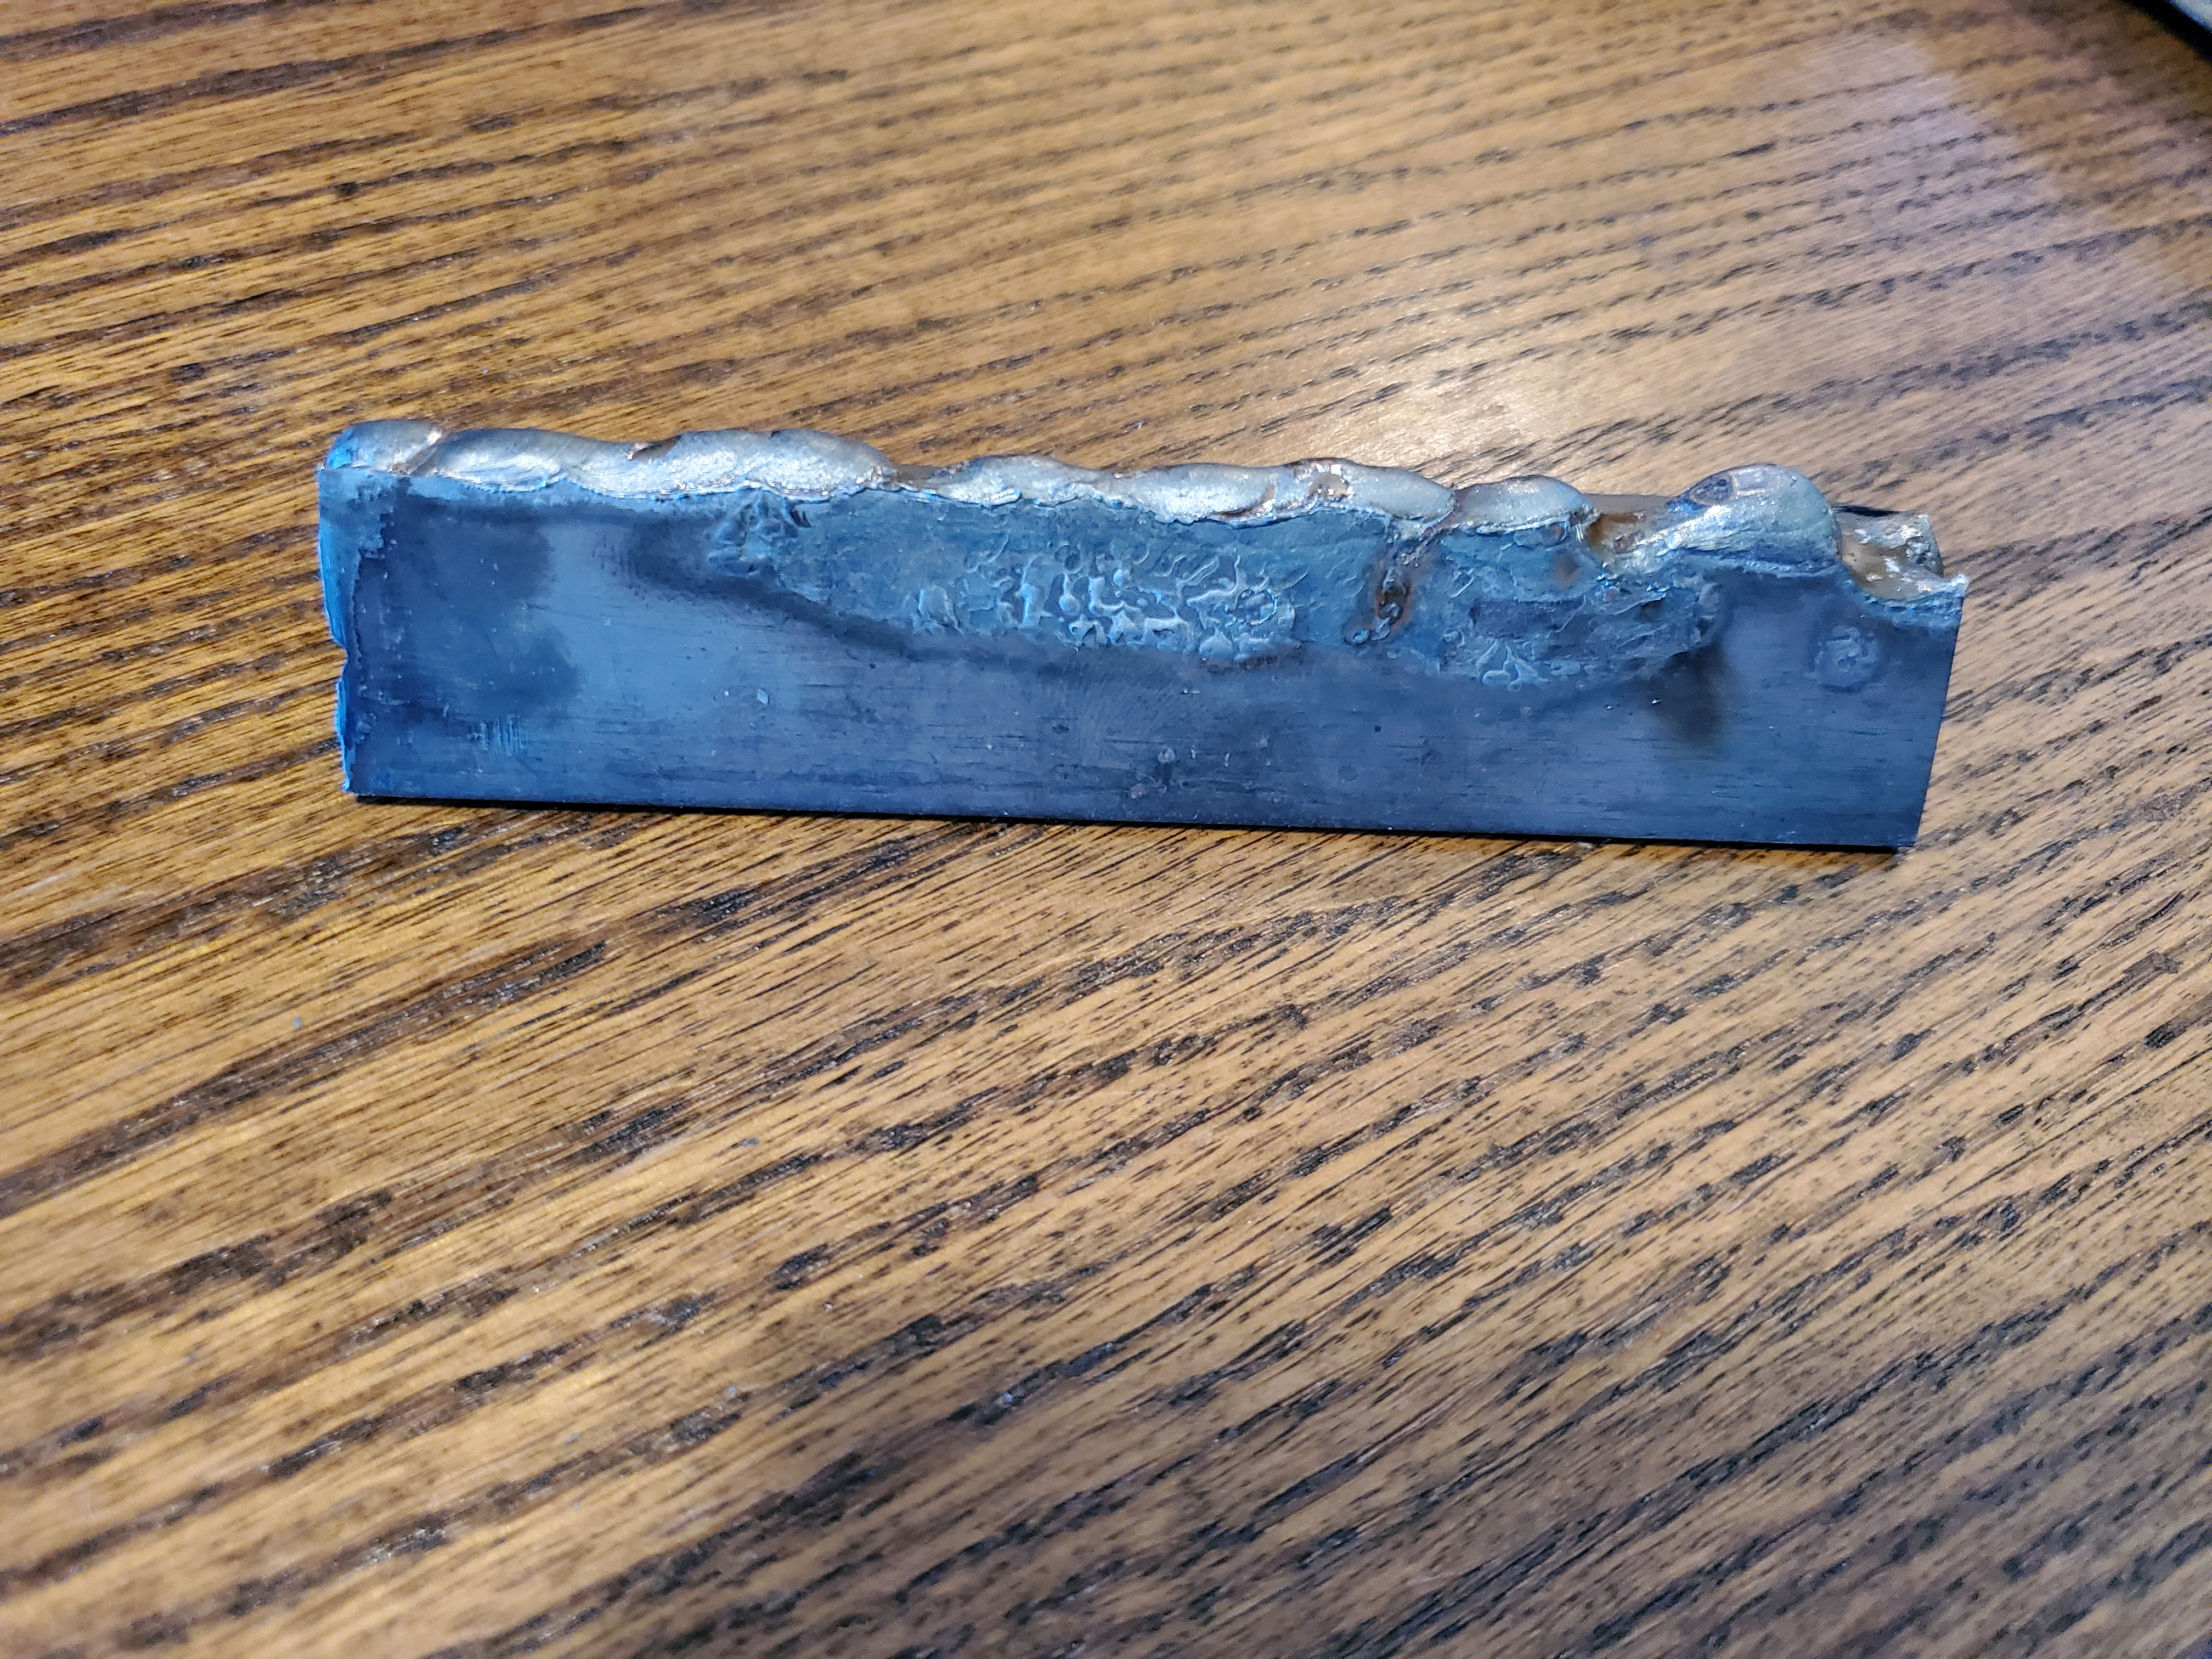
\includegraphics[width=\textwidth]{assets/cornerWeldOutside2_20240229.jpg}
\end{figure}

\subsection*{T Joint Weld}

\begin{figure}[h]
\caption{The front side of my T joint weld with the weld path running left to right between two tacks.}
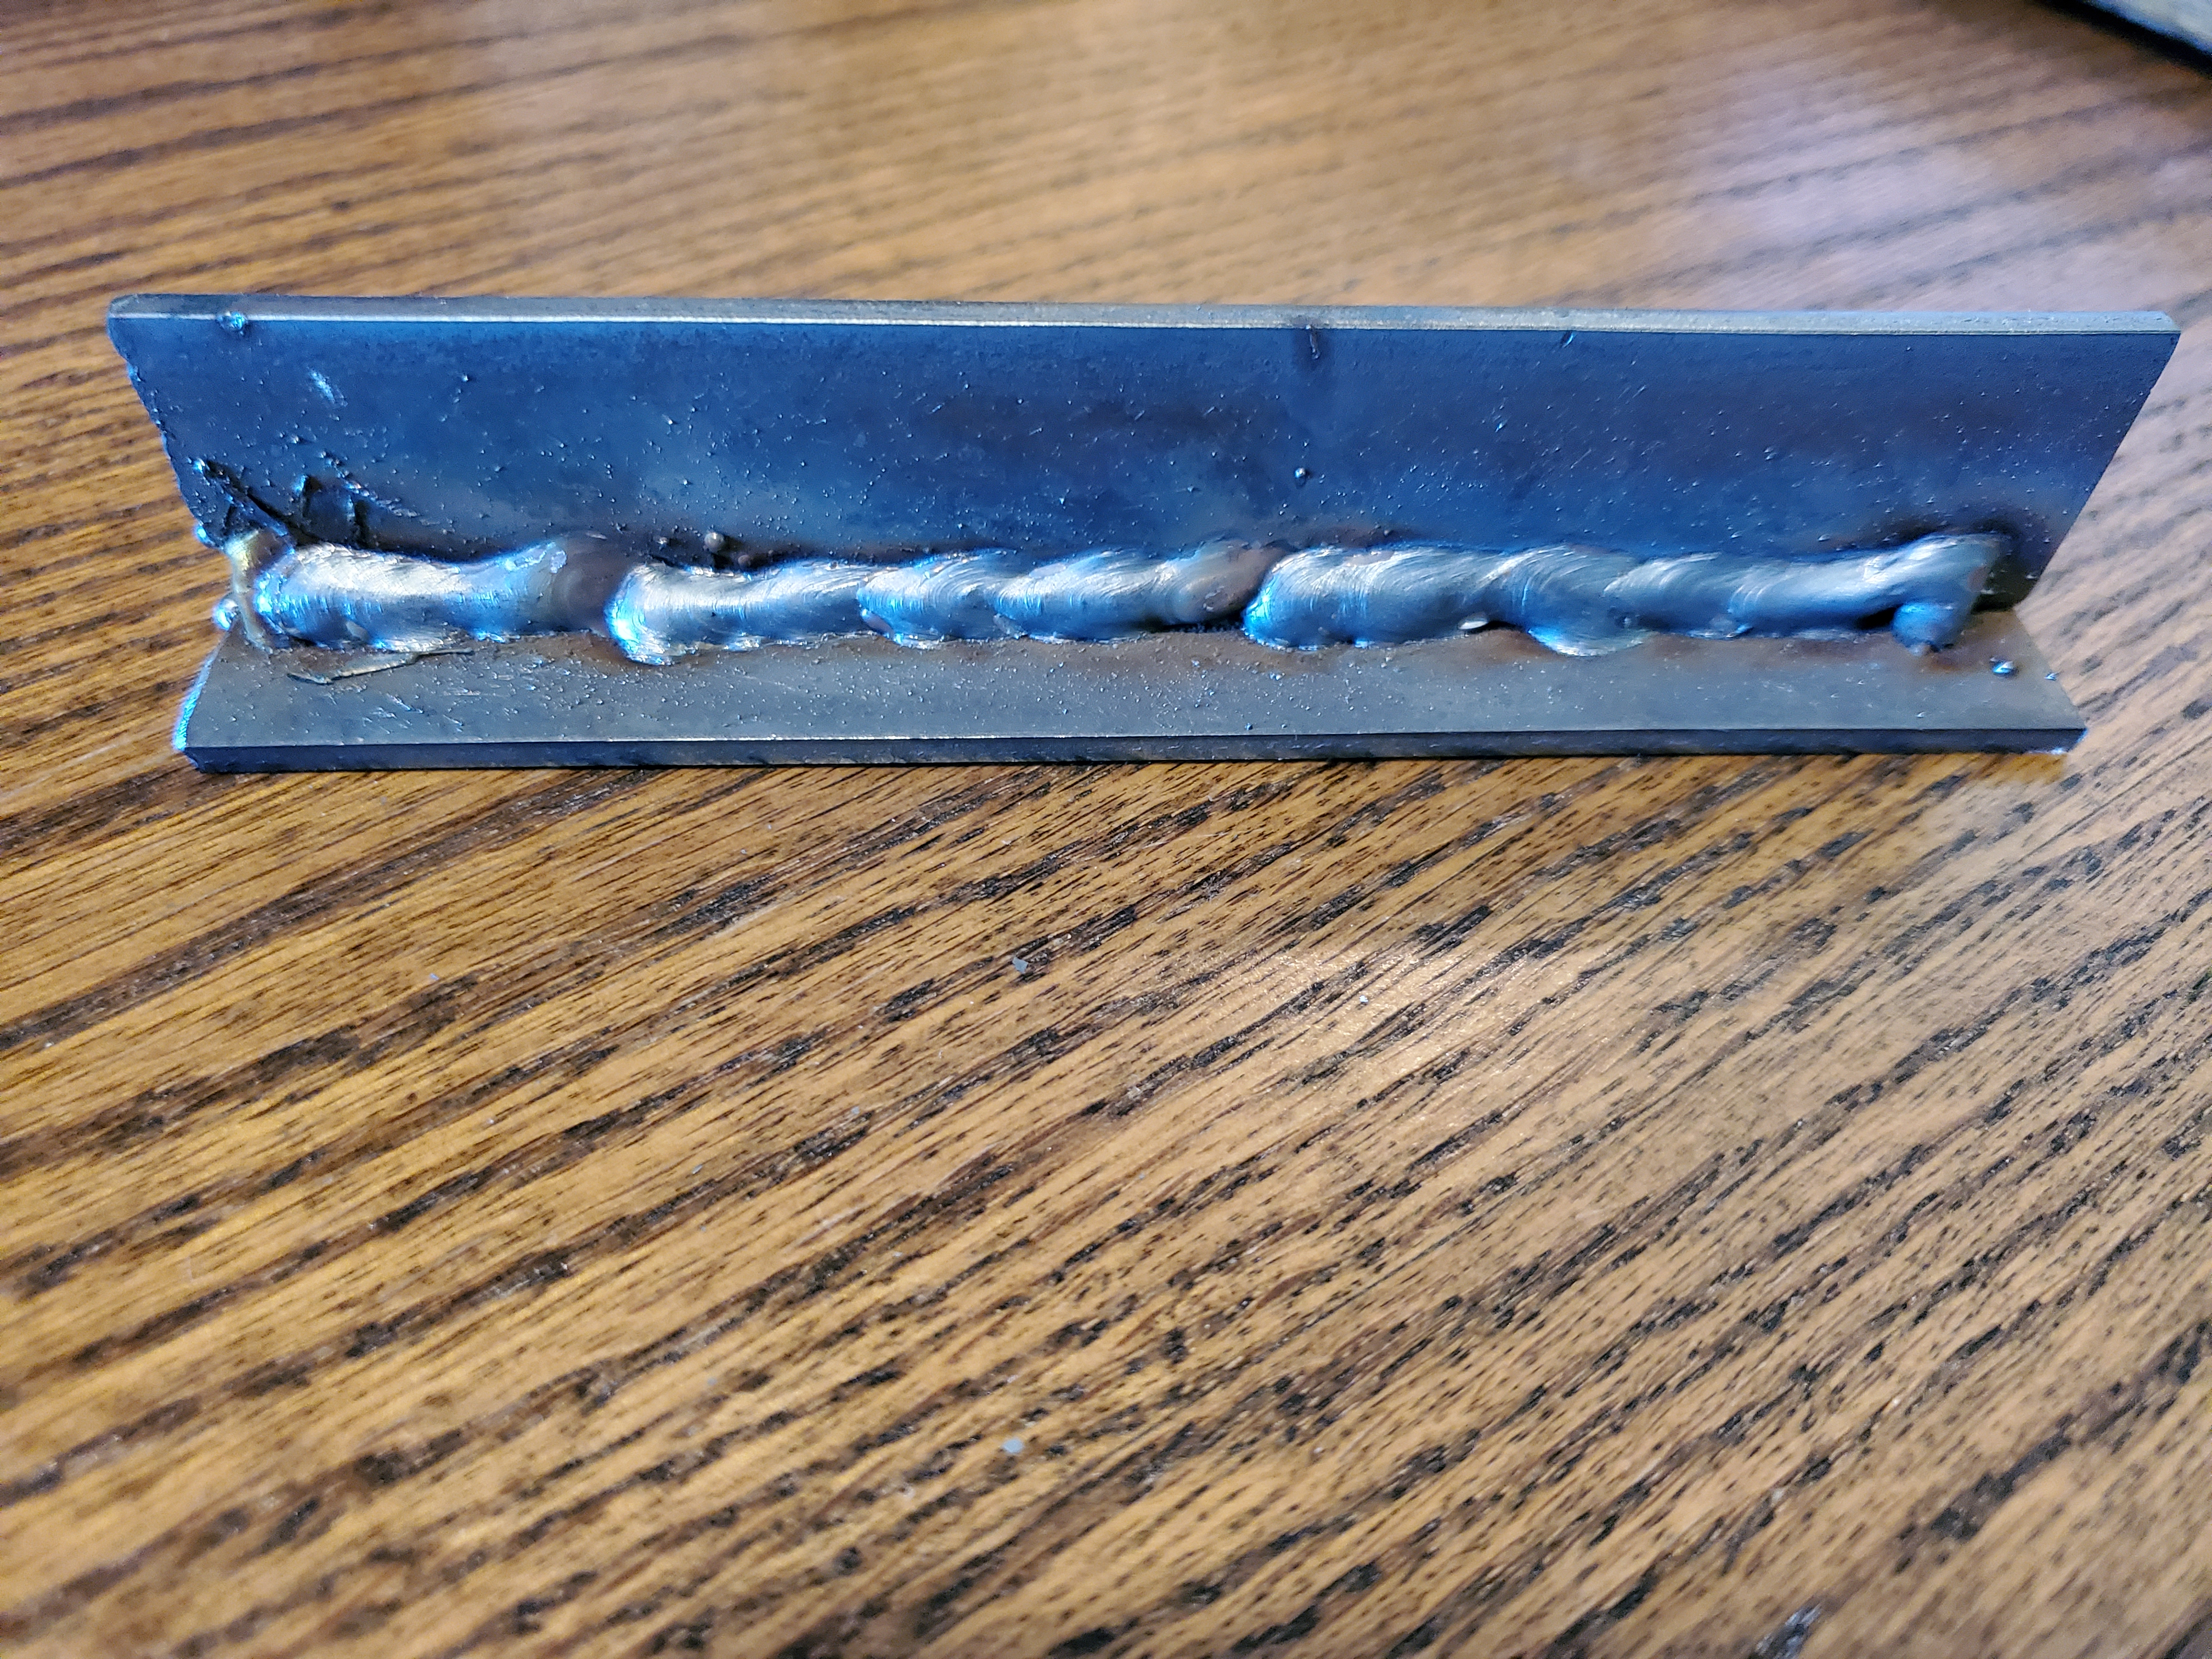
\includegraphics[width=\textwidth]{assets/tWeldFront_20240229.jpg}
\end{figure}

\begin{figure}[h]
\caption{The back side of my T join weld with the weld path running from left to right.}
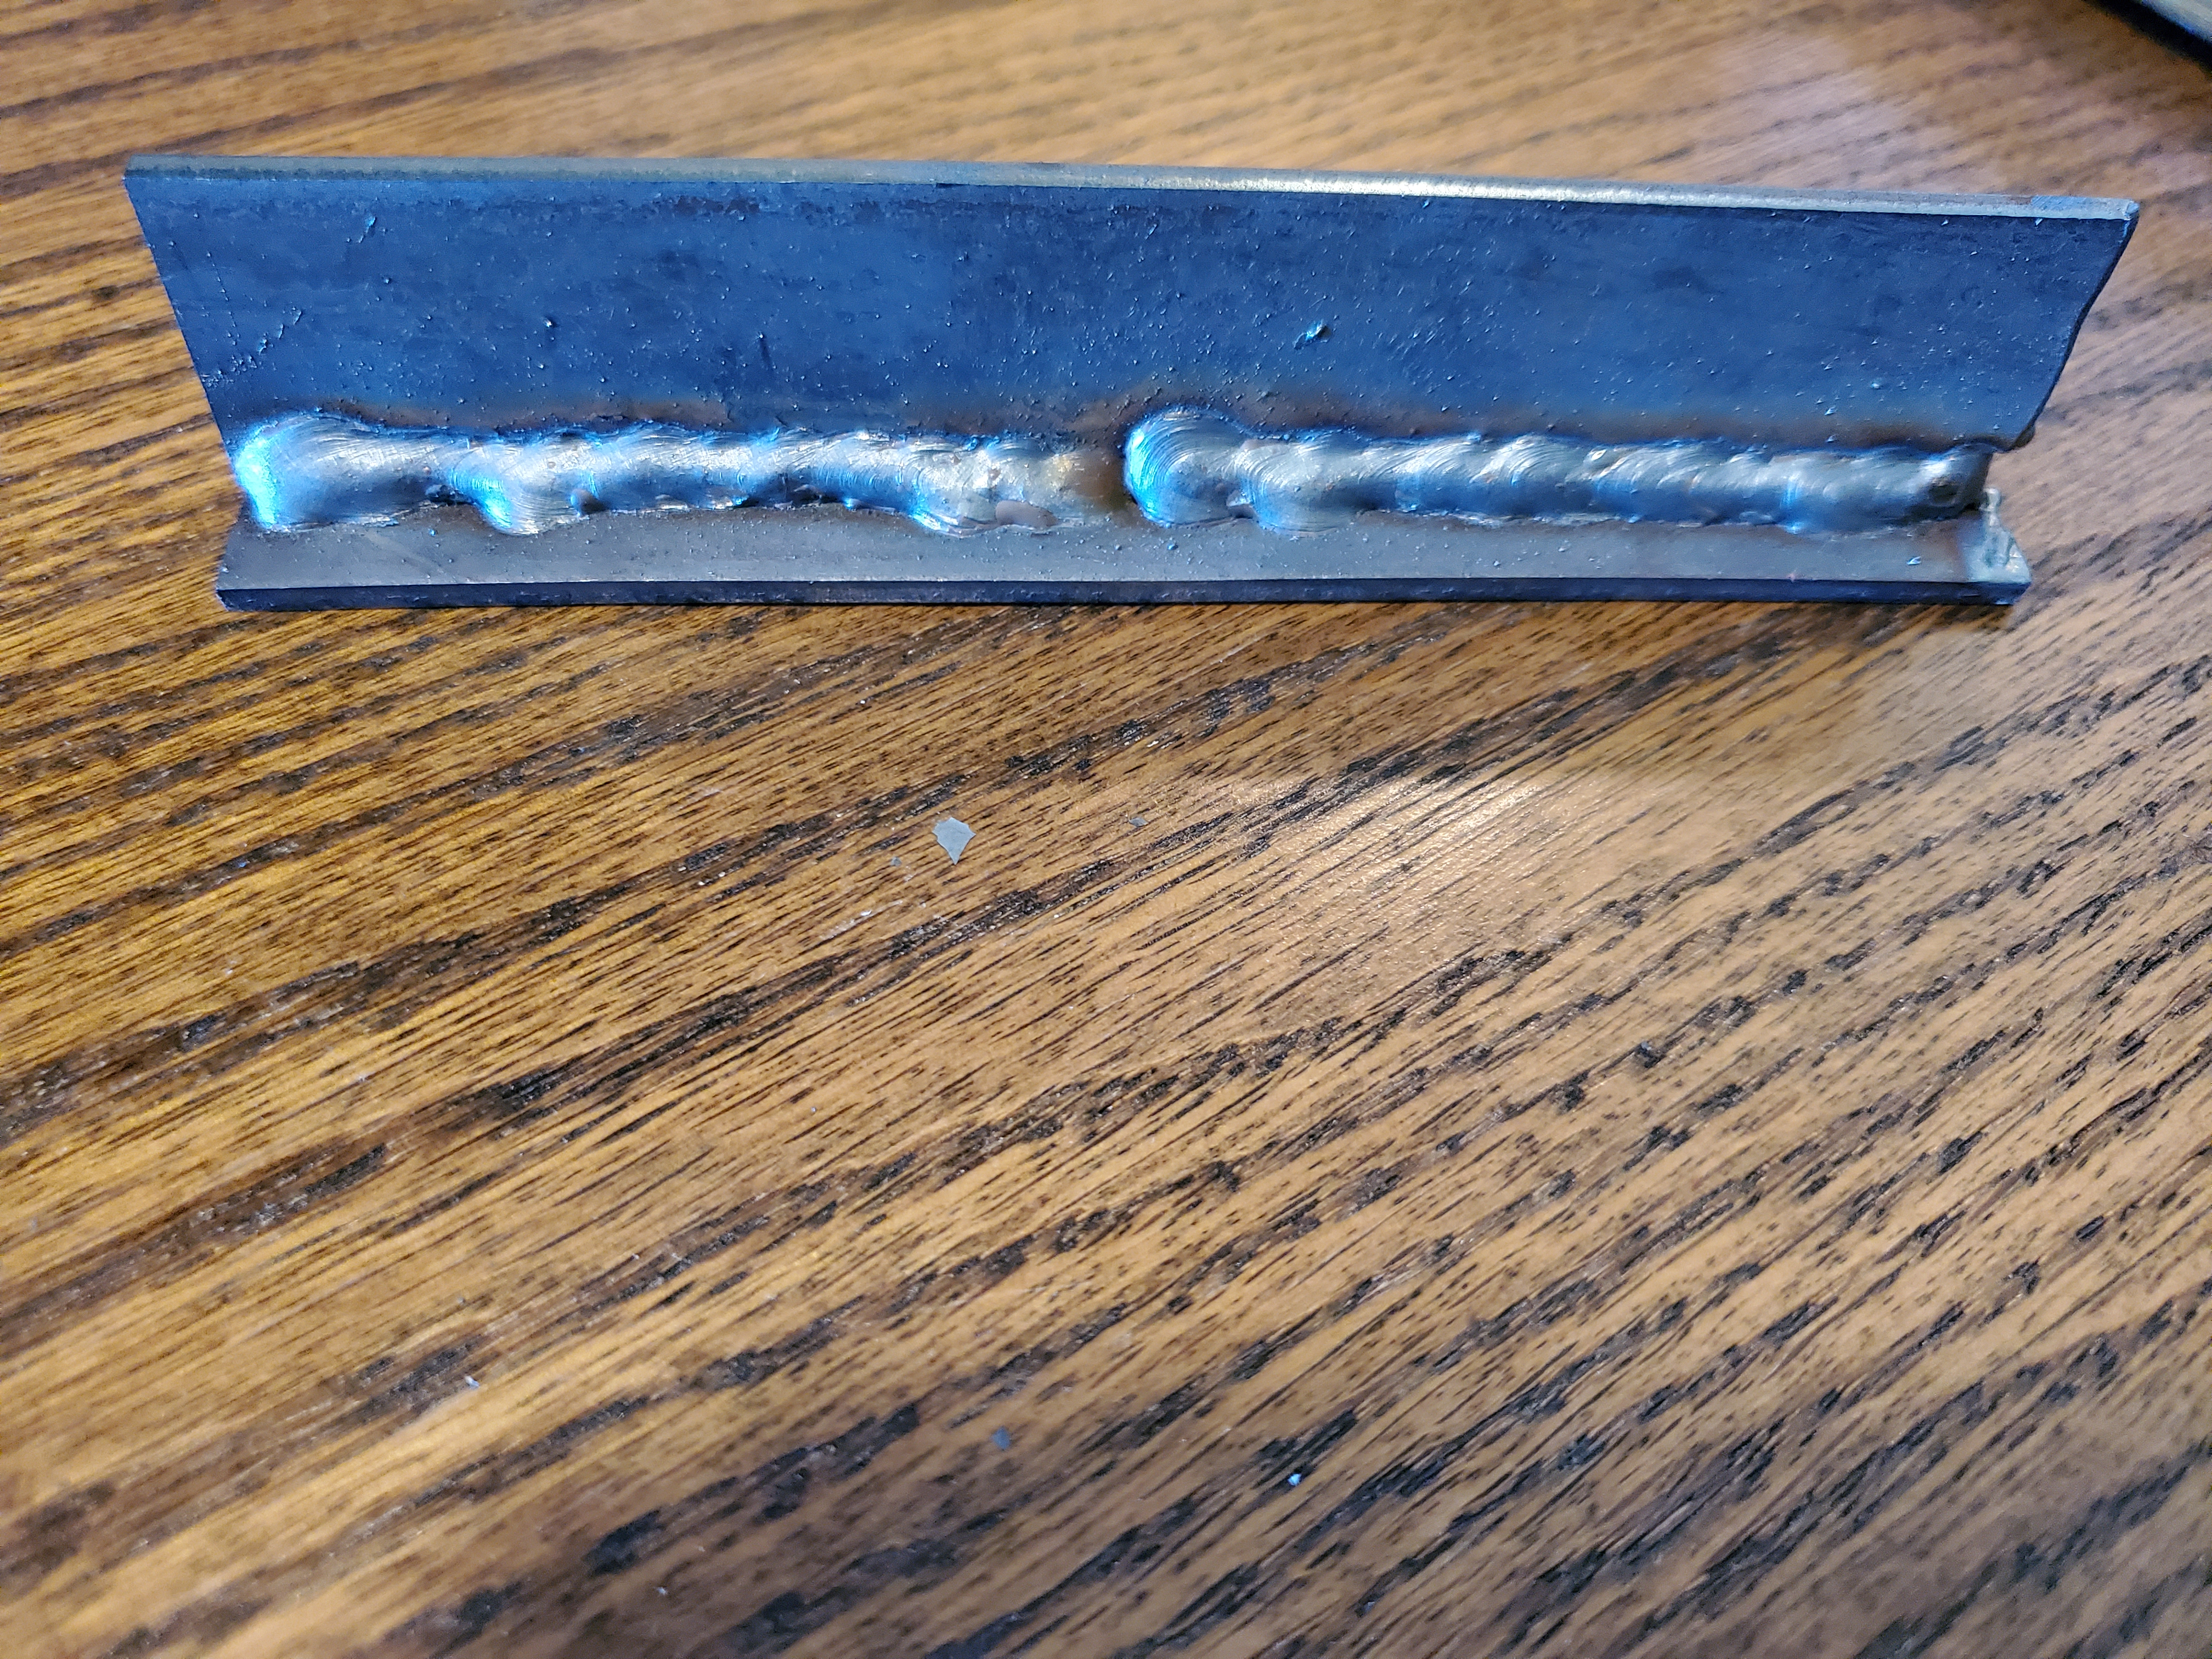
\includegraphics[width=\textwidth]{assets/tWeldBack_20240229.jpg}
\end{figure}

\section*{Final Thoughts}

I hope you enjoyed reading about my experience. I thought this was good fun, and I had to share. I had a wonderful time and learned so much from my awesome instructor, Dilip Patel, to whom I will also say thank you very much!

\end{document}
